% =======================================================================================
%   1. DOCUMENT SETUP & PACKAGES
% =======================================================================================
\documentclass[11pt, a4paper]{article}

% --- ESSENTIAL PACKAGES ---
\usepackage[utf8]{inputenc}
\usepackage[T1]{fontenc}
\usepackage[english]{babel}

% --- PAGE LAYOUT & STYLE ---
\usepackage[a4paper, margin=2.2cm, headheight=15pt, footskip=30pt]{geometry}
\usepackage{graphicx}
\usepackage{float}
\usepackage{caption}
\usepackage{subcaption}
\usepackage{fancyhdr}
\usepackage{xcolor}
\usepackage{titletoc}

% --- TYPOGRAPHY & TEXT ---
\usepackage{lato}
\renewcommand*\familydefault{\sfdefault}
\usepackage{textcomp}
\usepackage{fontawesome5}
\usepackage{microtype} % Improves line breaking and spacing

% Slightly more readable line spacing and allow more flexible breaks
\usepackage{setspace}
\setstretch{1.05}
\sloppy
\emergencystretch=2em

% --- TABLES, LISTS, & BOXES ---
\usepackage{booktabs}
\usepackage{longtable}
\usepackage{tabularx}
\usepackage{array}
\usepackage{enumitem}
\usepackage[skins, breakable, theorems]{tcolorbox}
\tcbuselibrary{skins, breakable, shadows} % Load advanced libraries

% --- TITLES & HYPERLINKS ---
\usepackage{titlesec}
\usepackage{hyperref} % Always load this last

% --- TIKZ FOR DIAGRAMS (STYLIZED WITH CORPORATE PALETTE) ---
\usepackage{tikz}
\usetikzlibrary{shapes, arrows.meta, positioning, shadows, calc, decorations.pathreplacing, backgrounds}
\usepackage{pgfkeys}

% =======================================================================================
%   2. COLOR & STYLE DEFINITIONS
% =======================================================================================

% --- CORPORATE COLOR PALETTE ---
\definecolor{WarlockRed}{HTML}{C11919}
\definecolor{WarlockGold}{HTML}{ECD125}
\definecolor{WarlockDark}{HTML}{1A1C1E}
\definecolor{WarlockGray}{HTML}{333333}
\definecolor{WarlockLightGray}{HTML}{F0F0F0}
\definecolor{WarlockWhite}{HTML}{FFFFFF}

% --- SECTION COLOR PALETTE ---
\definecolor{IntroColor}{HTML}{005A9B}      % Blue
\definecolor{QuickStartColor}{HTML}{00796B} % Green
\definecolor{InstallColor}{HTML}{8E44AD}    % Purple
\definecolor{ModelsColor}{HTML}{D35400}     % Orange
\definecolor{OptimizeColor}{HTML}{27AE60}   % Emerald Green
\definecolor{TroubleColor}{HTML}{C0392B}    % Red
\definecolor{ArchColor}{HTML}{2C3E50}       % Dark Blue
\definecolor{GlossaryColor}{HTML}{7F8C8D}   % Gray
\definecolor{SupportColor}{HTML}{34495E}    % Dark Gray

% --- TEXTBOX COLOR PALETTE ---
\definecolor{InfoFill}{HTML}{E7F3FE}
\definecolor{InfoBorder}{HTML}{005A9B}
\definecolor{WarnFill}{HTML}{FFFBE6}
\definecolor{WarnBorder}{HTML}{FFBE0B}
\definecolor{QuickStartFill}{HTML}{E6FFFA}
\definecolor{QuickStartBorder}{HTML}{00796B}

% --- DEFAULT TEXT COLOR APPLICATION ---
\color{WarlockGray}

% =======================================================================================
%   3. DOCUMENT ELEMENT CONFIGURATION
% =======================================================================================

% --- HYPERLINKS ---
\hypersetup{
    colorlinks=true,
    linkcolor=WarlockRed,
    filecolor=WarlockRed,
    urlcolor=WarlockRed,
    pdftitle={Warlock-Studio | Technical Documentation and User Manual},
    pdfauthor={Iván Eduardo Chavez Ayub}
}

% --- SECTION & SUBSECTION TITLES (CORRECTED) ---
\newcommand{\SectionColor}{WarlockGray} % Default color
\newcommand{\setsectioncolor}[1]{\renewcommand{\SectionColor}{#1}}

\titleformat{\section}
  {\normalfont\Large\bfseries}
  {}
  {0em}
  {%
    \begin{tcolorbox}[
        enhanced,
        colback=\SectionColor!90!black,
        colframe=\SectionColor!90!black,
        boxrule=0pt,
        sharp corners,
        halign=center,
        valign=center,
        boxsep=6pt,
        left=0pt, right=0pt, top=0pt, bottom=0pt
    ]
    \color{white}\faBookmark\hspace{0.5em}\thesection.\hspace{1em}#1
    \end{tcolorbox}
  }
\titleformat{\subsection}
  {\normalfont\large\bfseries\color{\SectionColor!80!black}}
  {\faCaretRight\ \thesubsection}
  {1em}
  {}
\titlespacing*{\section}{0pt}{4ex plus 1ex minus .2ex}{3ex plus .2ex}
\titlespacing*{\subsection}{0pt}{2.5ex plus 1ex minus .2ex}{1.3ex plus .2ex}

% --- ENHANCED TEXTBOX DEFINITIONS ---
\newtcolorbox{infobox}[2][]{
    enhanced, breakable,
    colback=InfoFill, colframe=InfoBorder,
    fonttitle=\bfseries, coltitle=InfoBorder,
    title=\faInfoCircle\hspace{0.5em}#2,
    attach boxed title to top left={yshift=-2mm, xshift=3mm},
    boxed title style={colback=InfoBorder, sharp corners},
    coltext=WarlockDark,
    shadow={2mm}{-1mm}{0mm}{black!20!white},
    #1
}
\newtcolorbox{warnbox}[2][]{
    enhanced, breakable,
    colback=WarnFill, colframe=WarnBorder,
    fonttitle=\bfseries, coltitle=WarnBorder!80!black,
    title=\faExclamationTriangle\hspace{0.5em}#2,
    attach boxed title to top left={yshift=-2mm, xshift=3mm},
    boxed title style={colback=WarnBorder, sharp corners},
    coltext=WarlockDark,
    shadow={2mm}{-1mm}{0mm}{black!20!white},
    #1
}
\newtcolorbox{quickstartbox}[2][]{
    enhanced, breakable,
    colback=QuickStartFill, colframe=QuickStartBorder,
    fonttitle=\bfseries, coltitle=QuickStartBorder!80!black,
    title=\faRocket\hspace{0.5em}#2,
    attach boxed title to top left={yshift=-2mm, xshift=3mm},
    boxed title style={colback=QuickStartBorder, sharp corners},
    coltext=WarlockDark,
    shadow={2mm}{-1mm}{0mm}{black!20!white},
    #1
}

% --- INLINE CODE COMMAND ---
% Use detokenize to preserve special characters and avoid problematic hyphenation
\newcommand{\inlinecode}[1]{\colorbox{WarlockLightGray}{\small\texttt{\detokenize{#1}}}}

% --- HEADER & FOOTER ---
\pagestyle{fancy}
\fancyhf{}
\fancyhead[L]{\textit{Warlock-Studio v4.3}}
\fancyhead[R]{\leftmark}
\fancyfoot[L]{\includegraphics[height=0.8cm]{logo.png}}
\fancyfoot[C]{\thepage}
\fancyfoot[R]{\textcopyright~2025 Warlock-Studio}
\renewcommand{\headrulewidth}{0.4pt}
\renewcommand{\footrulewidth}{0.4pt}
\renewcommand{\sectionmark}[1]{\markboth{\thesection. #1}{}}

% =======================================================================================
%   BEGIN DOCUMENT
% =======================================================================================
\begin{document}

% --- REDESIGNED TITLE PAGE (KEEPING ORIGINAL STYLE FROM YOUR BASE CODE) ---
\begin{titlepage}
    \begin{tcolorbox}[
        enhanced, sharp corners,
        colback=WarlockDark, colframe=WarlockGold,
        boxrule=2pt,
        height=\textheight,
        halign=center, valign=center
    ]
        \centering
        \includegraphics[width=0.4\textwidth]{logo.png}\par
        \vfill
        \color{WarlockWhite}
        {\Huge\bfseries\scshape Warlock-Studio\par}
        \vspace{1.5cm}
        \color{WarlockGold}
        \rule{0.6\textwidth}{1pt}\par
        \vspace{0.4cm}
        \color{WarlockWhite}
        {\Large\bfseries Technical Documentation and User Guide\par}
        \vspace{0.2cm}
        {\large Software Version: 4.3\par}
        \vspace{0.4cm}
        \color{WarlockGold}
        \rule{0.6\textwidth}{1pt}\par
        \vfill
        {\large Iván Eduardo Chavez Ayub\par}
        \href{https://github.com/Ivan-Ayub97}{\texttt{\color{WarlockGold}\faGithub\ @Ivan-Ayub97}}\par
        \vspace{1.5cm}
        {\large \today\par}
    \end{tcolorbox}
    \thispagestyle{empty}
\end{titlepage}

\newpage
\tableofcontents
\newpage

% =======================================================================================
%   SECTION 1: INTRODUCTION
% =======================================================================================
\setsectioncolor{IntroColor}
\section{Introduction to Warlock-Studio}
Welcome to Warlock-Studio — an AI-powered suite for digital media enhancement.  
It provides advanced tools for super-resolution, artifact removal, and frame generation through an intuitive interface that delivers professional-quality results with minimal effort.

% =======================================================================================
%   SECTION 2: QUICK START GUIDE
% =======================================================================================
\setsectioncolor{QuickStartColor}
\section{Quick Start Guide}
\begin{quickstartbox}{Accelerated Media Enhancement Procedure}
Follow these 5 steps to process your first media file in less than a minute.
\begin{enumerate}
    \item \textbf{Load Files:} Click the \textbf{"SELECT FILES"} button and choose one or more image or video files for processing.
    \item \textbf{AI Model Selection:} In the \textbf{"AI model"} dropdown menu, select an inference model.
    \begin{itemize}
        \item For photorealistic images, \inlinecode{BSRGANx4} is recommended for its ability to reconstruct fine textures.
        \item For animation or illustrated content, \inlinecode{RealESR_Animex4} is the optimal choice for preserving sharp edges.
        \item For video sequences, \inlinecode{RealESR_Gx4} offers an excellent balance between computational performance and perceptual quality.
    \end{itemize}
    \item \textbf{Adjust Input Resolution:} For a quick first pass, set \textbf{"Input resolution"} to \texttt{75}\%. This significantly reduces the computational load with an often imperceptible loss in final quality.
    \item \textbf{Verify VRAM Limit:} Ensure the value in \textbf{"GPU VRAM (GB)"} is equal to or less than your graphics card's dedicated video memory. An initial value of \texttt{4} GB is a safe setting for most modern hardware.
    \item \textbf{Start Processing:} Click \textbf{"Make Magic"} to initiate the processing pipeline. The output files will be generated in the specified directory or, by default, in the same location as the source files.
\end{enumerate}
\end{quickstartbox}

% =======================================================================================
%   SECTION 3: INSTALLATION & ARCHITECTURE
% =======================================================================================
\setsectioncolor{InstallColor}
\section{Installation and System Architecture}
\subsection{\faDownload\ Installation Process}
Warlock-Studio uses a self-contained offline installer, simplifying deployment.
\begin{enumerate}[leftmargin=*]
    \item \textbf{Obtaining the Executable:} Download the `Warlock-Studio-Setup.exe` file from the official repositories on GitHub or SourceForge.
    \item \textbf{Run with Elevated Privileges:} Right-click the installer and select "Run as administrator." This step is crucial to ensure the application has the necessary permissions to interact with low-level GPU drivers.
    \item \textbf{Installation Wizard:} Follow the on-screen instructions. The inclusion of all AI models and dependencies eliminates the need for additional downloads during this process.
    \item \textbf{Launch the Application:} Once the installation is complete, Warlock-Studio can be launched from the Start Menu or the desktop shortcut.
\end{enumerate}

\subsection{\faMicrochip\ System Requirements}
\begin{table}[H]
    \centering
    \begin{tabularx}{\textwidth}{lX}
        \toprule
        \textbf{Component} & \textbf{Technical Specification} \\
        \midrule
        Operating System & Windows 11 or Windows 10 (64-bit architecture required). \\
        RAM & 8 GB (minimum), 16 GB (recommended for high-resolution video processing). \\
        Graphics Card (GPU) & \textbf{Mandatory Requirement:} GPU with support for the \textbf{DirectX 12} API. \\
        & \textbf{NVIDIA (for CUDA):} Maxwell architecture (GTX 900 Series) or newer. Studio drivers are recommended for stability. \\
        & \textbf{AMD/Intel (for DirectML):} Any modern GPU with updated drivers that support DirectX 12 Feature Level 12.0+. \\
        & \textbf{4+ GB of VRAM} is recommended to avoid memory bottlenecks. \\
        Storage & 2 GB of free disk space. Using a Solid State Drive (SSD) drastically improves I/O performance during video sequence processing. \\
        \bottomrule
    \end{tabularx}
    \caption{Hardware and software specifications for optimal performance of Warlock-Studio.}
\end{table}

\subsection{\faFolderOpen\ File Structure and Dependencies}
\begin{infobox}{Self-Contained Components}
Warlock-Studio operates as a fully self-contained environment.  
All critical assets, dependencies, and user data are automatically managed by the application, requiring no manual configuration from the user.
\end{infobox}

\begin{itemize}[leftmargin=*]
    \item \textbf{Core Assets:}  
    The executables \inlinecode{ffmpeg.exe} (for video encoding/decoding) and \inlinecode{exiftool.exe} (for metadata preservation) are stored in the \texttt{Assets} directory.  
    Their paths are dynamically resolved through the \inlinecode{find_by_relative_path} function, which accurately locates resources in both development and bundled environments (using the \inlinecode{_MEIPASS} directory created by PyInstaller).

    \item \textbf{AI Models:}  
    All AI inference models are provided in interoperable \texttt{.onnx} format and stored within the \texttt{AI-onnx} directory.  
    This ensures cross-platform compatibility and seamless hardware acceleration through ONNX Runtime.

    \item \textbf{User Preferences:}  
    The configuration file \inlinecode{USER_PREFERENCE_PATH} is automatically generated in the user’s \textbf{Documents} folder (\inlinecode{os_path_expanduser('~')}).  
    It stores GUI layout, last-used settings, and model selections between sessions.

    \item \textbf{Diagnostic Logs:}  
    Log files (\inlinecode{MAIN_LOG_FILENAME} and \inlinecode{ERROR_LOG_FILENAME}) are created in a dedicated subfolder inside \textbf{Documents}.  
    These serve as vital diagnostic resources, recording operational events, system validation reports, and runtime exceptions for troubleshooting.
\end{itemize}


% =======================================================================================
%   SECTION 4: DETAILED AI MODEL GUIDE
% =======================================================================================
\setsectioncolor{ModelsColor}
\section{Detailed Analysis of Inference Models}

\begin{infobox}{Model Selection Overview}
Selecting the appropriate AI inference model is the most critical decision 
in Warlock-Studio’s enhancement pipeline. It directly determines the balance 
between visual quality, computational efficiency, and hardware resource usage. 
Each model implements distinct neural architectures and loss functions, optimized 
for different types of input data and output fidelity targets.

The following section provides a comprehensive technical breakdown and comparative 
analysis to support informed model selection.
\end{infobox}


\subsection{\faTable\ Model Comparison Matrix}
\begin{longtable}{p{2.8cm} p{1.8cm} p{1.2cm} p{1.5cm} p{7.2cm}}
\toprule
\textbf{Model} & \textbf{Primary Function} & \textbf{Scale} & \textbf{VRAM (GB)} & \textbf{Use Case and Technical Considerations} \\
\midrule
\endhead
\multicolumn{5}{c}{\textit{\textbf{\faEraser\ Denoising Models}}} \\
\midrule
\texttt{IRCNN\_Mx1} & Denoise & x1 & 4.0 & Moderate-level noise reduction. Ideal for suppressing JPEG compression artifacts and low-ISO sensor noise in old photographs. \\
\texttt{IRCNN\_Lx1} & Denoise & x1 & 4.0 & Intensive noise reduction algorithm. Optimal for severely degraded images with pronounced luminance and chrominance noise. \\
\midrule
\multicolumn{5}{c}{\textit{\textbf{\faTachometerAlt\ High-Fidelity Upscaling Models (Computationally Intensive)}}} \\
\midrule
\texttt{BSRGANx4} & Upscale & x4 & 0.6 & Generative Adversarial Network optimized for realistic texture synthesis. It is the model of choice for portraits, nature photography, and where the preservation of fine details is paramount. \\
\texttt{BSRGANx2} & Upscale & x2 & 0.7 & A variant with a reduced scaling factor. It offers a perceptual quality similar to the x4 version but with lower computational cost, ideal for moderate upscaling needs. \\
\texttt{RealESRGANx4} & Upscale & x4 & 0.6 & A robust general-purpose model. It excels in reconstructing a wide variety of content, including textures, landscapes, and architectural elements. \\
\texttt{RealESRNetx4} & Upscale & x4 & 2.2 & An alternative to RealESRGAN, often producing results with fewer "hallucinatory" artifacts. It can offer a better balance between speed and fidelity on certain GPU architectures. \\
\midrule
\multicolumn{5}{c}{\textit{\textbf{\faBolt\ High-Speed Upscaling Models (Lightweight)}}} \\
\midrule
\texttt{RealESR\_Gx4} & Upscale & x4 & 2.2 & A lightweight and fast model, optimized for real-time or near-real-time video processing. It offers an excellent compromise between performance and visual quality. \\
\texttt{RealESR\_Animex4} & Upscale & x4 & 2.2 & Specialized for non-photorealistic content. It preserves sharp lines and flat colors, avoiding the smoothing artifacts common in models trained on natural data. \\
\midrule
\multicolumn{5}{c}{\textit{\textbf{\faUserCircle\ Facial Restoration Models}}} \\
\midrule
\texttt{GFPGAN} & Restore & x1 & 1.8 & Generative Adversarial Network with a facial prior. It not only upscales but also reconstructs and enhances damaged or low-resolution facial features in photographs. \\
\midrule
\multicolumn{5}{c}{\textit{\textbf{\faFilm\ Frame Interpolation Models (Video Only)}}} \\
\midrule
\texttt{RIFE} & Interpolate & N/A & \textasciitilde{}1.5 & High-quality algorithm for motion interpolation. It generates intermediate frames to increase the fluidity of a video (e.g., from 30 to 60 FPS). \\
\texttt{RIFE\_Lite} & Interpolate & N/A & \textasciitilde{}1.2 & An optimized variant of RIFE, designed for GPUs with limited VRAM. It offers faster processing at the cost of a slight reduction in interpolation accuracy. \\
\midrule
\bottomrule
\caption{Technical guide for the selection of AI models. VRAM values are base estimates derived from the \inlinecode{VRAM_model_usage} dictionary in the source code and may vary.}
\label{tab:modelos}
\end{longtable}

% =======================================================================================
%   SECTION 5: BEST PRACTICES & OPTIMIZATION
% =======================================================================================
\setsectioncolor{OptimizeColor}
\section{Performance Optimization and Best Practices}

\subsection{\faSlidersH\ Critical Performance Parameters}
\begin{itemize}[leftmargin=*, itemsep=2pt]
    \item \textbf{Input Resolution \%:} This is the most influential parameter on processing speed. A value between \textbf{50\% and 75\%} implements an initial downsampling before upscaling, drastically reducing the computational load with minimal impact on the final perceptual quality.
    
\item \textbf{GPU VRAM Limiter (GB):} Defines the video memory budget. 
This value (from \inlinecode{selected_VRAM_limiter.get()}) is used in a precise formula 
to calculate the internal \inlinecode{tiles_resolution} parameter:

\begin{center}
\begin{tcolorbox}[
    enhanced,
    colback=WarlockLightGray!30,
    colframe=OptimizeColor!80!black,
    boxrule=0.6pt,
    arc=2pt,
    left=4pt,right=4pt,top=2pt,bottom=2pt,
    width=0.9\linewidth
]
\small
\texttt{vram\_factor = VRAM\_model\_usage[model] * VRAM\_GB\_input}\\
\texttt{tiles\_resolution = int(vram\_factor * 100)}
\end{tcolorbox}
\end{center}

This \inlinecode{tiles_resolution} (e.g., \texttt{880px} for a 4~GB card using 
\inlinecode{RealESR_Gx4}) is then used as the maximum tile dimension for image processing, 
ensuring full stability and preventing \textbf{Out Of Memory (OOM)} errors during inference.

    
    \item \textbf{AI Multithreading:} (Video only) Allows for the parallel processing of multiple frames via a \inlinecode{ThreadPool}. It significantly increases performance on systems with multi-core CPUs, but at the cost of higher VRAM and CPU consumption.
    
    \item \textbf{AI Blending:} Mitigates visual artifacts. This value (from \inlinecode{selected_blending_factor}) is passed to the \inlinecode{blend_images_and_save} function, which uses OpenCV's \inlinecode{addWeighted} to perform an alpha blend between the original upscaled image and the AI-processed image.

    \item \textbf{System Validation:} Before starting, the \inlinecode{validate_system_requirements} function automatically checks for the presence of \inlinecode{ffmpeg.exe}, available disk space, and available system RAM (using the \inlinecode{psutil} library).
\end{itemize}
\subsection{\faTrophy\ Tips for Maximum Quality Results}

\begin{tcolorbox}[
    enhanced, breakable,
    colback=QuickStartFill,
    colframe=QuickStartBorder,
    coltitle=QuickStartBorder!80!black,
    title=\faStar\hspace{0.5em}\textbf{Expert Recommendations for Optimal Output},
    fonttitle=\bfseries,
    sharp corners,
    boxrule=0.6pt,
    shadow={1mm}{-1mm}{0mm}{black!10!white}
]

\begin{description}[leftmargin=*, style=nextline, itemsep=1em]

    \item[\textbf{Maximizing Visual Fidelity}]
    To achieve the highest possible perceptual quality, use the \inlinecode{BSRGANx4} or \inlinecode{RealESRGANx4} models with an \textbf{Input Resolution} of \textbf{100\%}.  
    Although computationally demanding, this configuration ensures maximum reconstruction of micro-textures and reduces information loss, especially on portrait or landscape imagery.

    \item[\textbf{Workflow for Video Restoration}]
    A robust two-stage restoration pipeline for archival or degraded footage involves:  
    \begin{enumerate}[nosep, leftmargin=*]
        \item \textbf{Stage 1 — Denoising:} Apply a denoising model such as \inlinecode{IRCNN\_Mx1} to clean sensor noise and compression artifacts.  
        \item \textbf{Stage 2 — Upscaling:} Use an upscaling model such as \inlinecode{RealESR\_Gx4} on the cleaned output to reconstruct fine detail while maintaining temporal coherence.
    \end{enumerate}

    \item[\textbf{Impact of SSD Storage}]
    A Solid State Drive (SSD) significantly improves throughput during video restoration.  
    The extraction (\inlinecode{extract\_video\_frames}), writing (\inlinecode{save\_frames\_on\_disk}), and reassembly (\inlinecode{video\_encoding}) of thousands of frames represent the main I/O bottlenecks; SSDs mitigate these delays and improve system responsiveness.

    \item[\textbf{Frame Persistence for Experimentation}]
    For testing different encoding settings (e.g., codecs or bitrates), enable the \textbf{"Keep frames"} option (\inlinecode{selected\_keep\_frames = True}).  
    This preserves the processed frames on disk, allowing video re-encoding without repeating the AI inference phase — saving time and extending the experimental workflow.

\end{description}
\end{tcolorbox}


% =======================================================================================
%   SECTION 6: TROUBLESHOOTING
% =======================================================================================
\setsectioncolor{TroubleColor}
\section{Diagnostics and Troubleshooting}
\begin{warnbox}{Primary Cause of Errors}
The \textbf{\#1 cause} of processing failures is \textbf{non-standard characters} in file paths and filenames. Avoid using: \texttt{', ", @, \#, \$, \%, \&, *, [, ], ?, etc.}.
\end{warnbox}

\begin{description}[leftmargin=*, style=nextline, itemsep=0.8em]
    \item[\faBan\ Error: "FFmpeg encoding failed..."]
        \textbf{Diagnosis:} The \inlinecode{video_encoding} function, which uses \inlinecode{subprocess_run}, has failed. The code specifically checks for several causes:
        \begin{itemize}[nosep, leftmargin=*]
            \item \textbf{"Invalid argument"}: Most commonly caused by special characters in file paths.
            \item \textbf{"Unknown encoder"}: The selected video codec (e.g., \inlinecode{hevc_nvenc}) is not supported by your FFmpeg build or hardware.
            \item \textbf{"Device or resource busy"}: Your GPU's hardware encoder is being used by another application (e.g., OBS, ShadowPlay).
        \end{itemize}
        \textbf{Solution:} Rename files to remove special characters. For encoder errors, select a different codec (e.g., \inlinecode{x264} or \inlinecode{x265}).

    \item[\faRocket\ Error: "Failed to load model" or Execution Provider Failure]
        \textbf{Diagnosis:} Failure in the initialization of the selected hardware backend, caught within the \inlinecode{create_onnx_session} function.
        \textbf{Solution:} The system is designed to automatically fall back to a functional provider in the hierarchy (CUDA -> DirectML -> CPU). To resolve the root cause:
        \begin{enumerate}[nosep, leftmargin=*]
            \item \textbf{For CUDA errors:} Verify the installation of the latest NVIDIA drivers (Game Ready or Studio).
            \item \textbf{For DirectML errors:} Ensure that the Windows operating system is fully updated and that you have the latest drivers for your GPU (NVIDIA, AMD, or Intel).
        \end{enumerate}

    \item[\faMemory\ Error: "out of memory" (OOM) or "allocation" failure]
        \textbf{Diagnosis:} The GPU's VRAM has been exhausted. This error is caught within the \inlinecode{upscale_video_frames_async} function.
        \textbf{Solution:}
        \begin{enumerate}[nosep, leftmargin=*]
            \item Lower the \textbf{VRAM Limiter} to a value equal to or less than your GPU's physical VRAM.
            \item Decrease the \textbf{Input Resolution \%} to 75\% or less.
            \item \textbf{Automatic Recovery:} The code will attempt an automatic recovery. It progressively reduces the processing tile size (by lowering the \inlinecode{AI_instance.max_resolution} variable) and retries the failed frame.
        \end{enumerate}

    \item[\faTachometerAlt\ Error: "cannot convert float NaN to integer"]
        \textbf{Diagnosis:} This specific error is caught in the main \inlinecode{upscale_orchestrator}. It indicates a GPU driver timeout (TDR - Timeout Detection and Recovery), often caused by hardware overload or overheating, which returns a "Not a Number" (NaN) value instead of pixel data.
        \textbf{Solution:} Restart the process \textbf{without deleting the generated frames folder}. The application will detect the existing frames and resume the task from the point of failure.
\end{description}

% =======================================================================================
%   SECTION 7: ADVANCED TECHNICAL ARCHITECTURE
% =======================================================================================
\setsectioncolor{ArchColor}
\section{Software Architecture Analysis}

\subsection{\faCogs\ Inference Engine and Hardware Abstraction}
Warlock-Studio is built upon a multi-layered inference engine powered by \textbf{ONNX Runtime}. The \inlinecode{create_onnx_session} function abstracts the underlying hardware and prioritizes Execution Providers to maximize performance:
\begin{enumerate}[leftmargin=*]
    \item \textbf{CUDA (\texttt{CUDAExecutionProvider}):} The highest performance option, leveraging the parallel computing architecture of NVIDIA GPUs.
    \item \textbf{DirectML (\texttt{DmlExecutionProvider}):} If CUDA is not available, the system falls back to DirectML. This Microsoft API translates neural network operations into native \textbf{DirectX 12} calls, ensuring broad hardware compatibility (NVIDIA, AMD, Intel).
    \item \textbf{CPU (\texttt{CPUExecutionProvider}):} This is the last resort provider. If no GPU acceleration is viable, the application runs the model on the CPU, guaranteeing universal functionality at the cost of significantly lower performance.
\end{enumerate}

\subsection{\faThLarge\ Dynamic Tiling and Memory Management}
To process high-resolution media, the \inlinecode{AI_upscale_with_tilling} function is invoked. It programmatically subdivides a large frame into smaller "tiles" based on the \inlinecode{max_resolution} variable. This \inlinecode{max_resolution} (confusingly named \inlinecode{tiles_resolution} in the GUI logic) is the pixel dimension calculated directly from the user's \textbf{VRAM Limiter} input, ensuring that no single tile exceeds the GPU's memory budget.

\subsection{\faSyncAlt\ Resume and Checkpointing Functionality}
If a video process is interrupted, the frames already processed and written to disk are preserved. Upon restarting the same task, the \inlinecode{check_video_upscaling_resume} function detects these partial files by checking for their existence. It then returns a list of only the *original* frames that still need processing, allowing the \inlinecode{upscale_video} orchestrator to resume the task from the point of failure.

\subsection{\faBolt\ Asynchronous Frame Writing}
During video upscaling, the main processing loop in \inlinecode{upscale_video_frames_async} does not write to disk directly. Instead, it batches processed frames in memory. Once a batch is ready (defaulting to \inlinecode{MULTIPLE_FRAMES_TO_SAVE = 8}), it calls \inlinecode{save_frames_on_disk}, which spawns a new \inlinecode{Thread} from the `threading` module to run \inlinecode{save_multiple_upscaled_frame_async}. This decouples the GPU-bound inference from the I/O-bound disk writing, maximizing GPU utilization.

% =======================================================================================
%   SECTION 8: PROCESSING PIPELINE DIAGRAM (FIXED TO PAGE WIDTH)
% =======================================================================================
\section{Processing Pipeline (Diagram)}
\noindent
The following diagram illustrates the high-level processing pipeline.

\begin{figure}[H]
    \centering
    % Resize to text width to avoid overflow
    \resizebox{\textwidth}{!}{%
    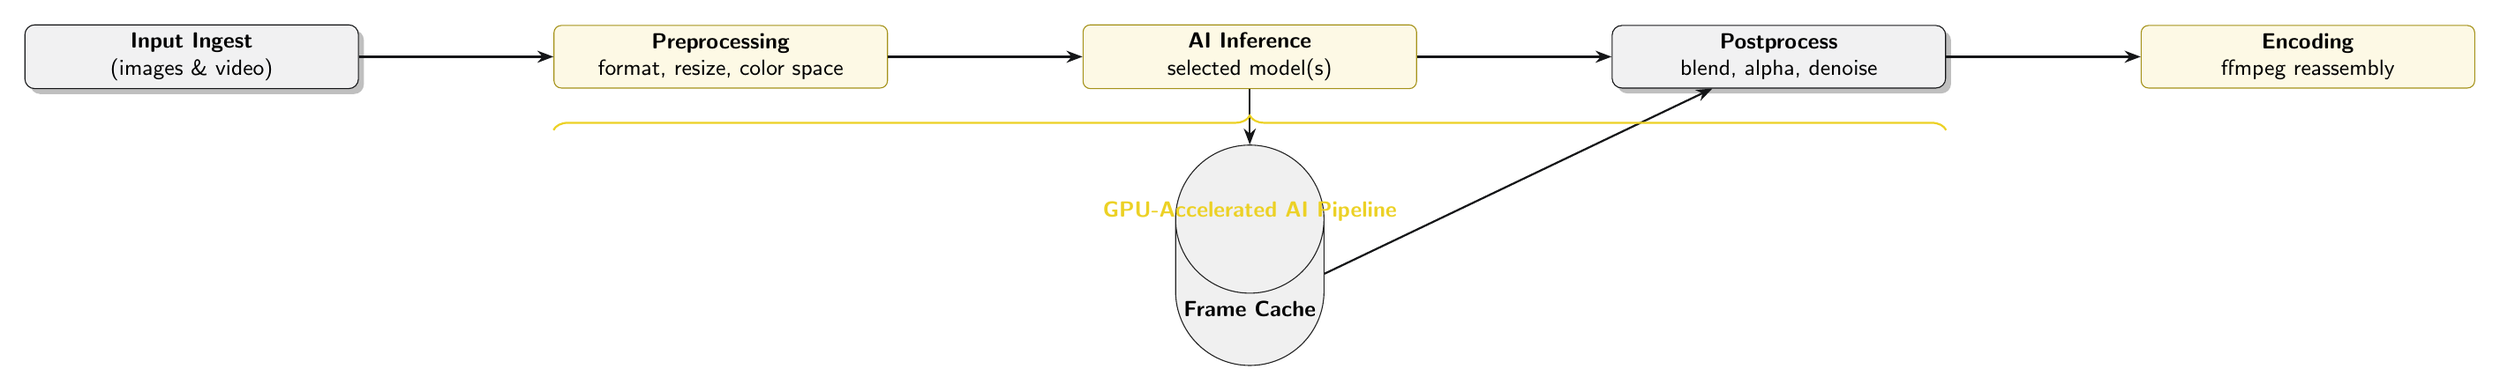
\begin{tikzpicture}[node distance=12mm, every node/.style={font=\small}, >=Stealth]
      \tikzset{
        box/.style={rectangle, rounded corners=4pt, draw=WarlockDark!80!black, fill=WarlockDark!6, minimum width=48mm, minimum height=9mm, align=center, drop shadow},
        proc/.style={rectangle, rounded corners=3pt, draw=WarlockGold!70!black, fill=WarlockGold!12, minimum width=48mm, minimum height=9mm, align=center},
        disk/.style={cylinder, shape border rotate=90, draw=WarlockGray!70!black, fill=WarlockLightGray, minimum width=10mm, minimum height=10mm, align=center},
        arrow/.style={->, thick, draw=WarlockDark!80!black}
      }
      \node[box] (ingest) {\textbf{Input Ingest}\\(images \& video)};
      \node[proc, right=28mm of ingest] (analysis) {\textbf{Preprocessing}\\format, resize, color space};
      \node[proc, right=28mm of analysis] (model) {\textbf{AI Inference}\\selected model(s)};
      \node[box, right=28mm of model] (post) {\textbf{Postprocess}\\blend, alpha, denoise};
      \node[disk, below=8mm of model] (cache) {\textbf{Frame Cache}};
      \node[proc, right=28mm of post] (encode) {\textbf{Encoding}\\ffmpeg reassembly};

      \draw[arrow] (ingest) -- (analysis);
      \draw[arrow] (analysis) -- (model);
      \draw[arrow] (model) -- (post);
      \draw[arrow] (post) -- (encode);
      \draw[arrow] (model) -- (cache);
      \draw[arrow] (cache) -- (post);

      % Decorative bracket and label under pipeline
      \draw[decorate, decoration={brace, amplitude=6pt}, thick, WarlockGold] ($(analysis.south west)+(0,-6mm)$) -- ($(post.south east)+(0,-6mm)$) node[midway, below=9mm]{\small \textbf{GPU-Accelerated AI Pipeline}};
    \end{tikzpicture}
    }
    \caption{High-level processing pipeline (ingest $\rightarrow$ inference $\rightarrow$ encode).}
\end{figure}

% =======================================================================================
%   SECTION 10: ARCHITECTURE DIAGRAM (FIXED)
% =======================================================================================
\section{Software Architecture (Diagram)}
\noindent
Component-level architecture showing logical components and their relationship to hardware.

\begin{figure}[H]
    \centering
    \resizebox{\textwidth}{!}{%
    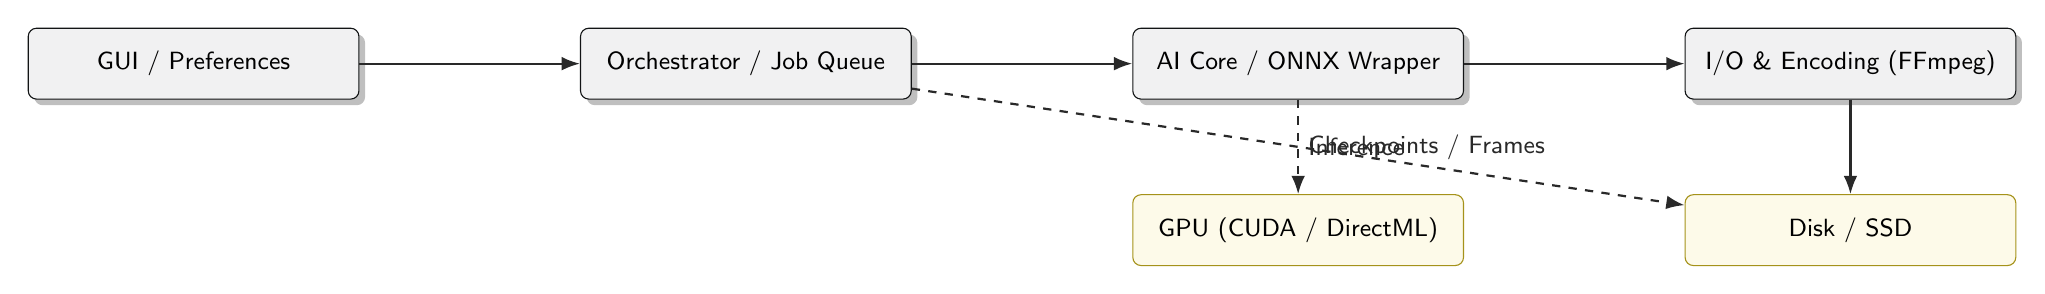
\begin{tikzpicture}[node distance=12mm, every node/.style={font=\small}]
      \tikzset{
        comp/.style={rectangle, rounded corners=3pt, draw=WarlockDark!70!black, fill=WarlockDark!6, minimum width=42mm, minimum height=9mm, align=center, drop shadow},
        hw/.style={rectangle, rounded corners=3pt, draw=WarlockGold!70!black, fill=WarlockGold!10, minimum width=42mm, minimum height=9mm, align=center},
        line/.style={-Latex, thick, color=WarlockGray!80!black}
      }
      \node[comp] (gui) {GUI / Preferences};
      \node[comp, right=28mm of gui] (orchestrator) {Orchestrator / Job Queue};
      \node[comp, right=28mm of orchestrator] (ai) {AI Core / ONNX Wrapper};
      \node[comp, right=28mm of ai] (io) {I/O \& Encoding (FFmpeg)};
      \node[hw, below=12mm of ai] (gpu) {GPU (CUDA / DirectML)};
      \node[hw, below=12mm of io] (disk) {Disk / SSD};

      \draw[line] (gui) -- (orchestrator);
      \draw[line] (orchestrator) -- (ai);
      \draw[line] (ai) -- (io);
      \draw[line, dashed] (ai) -- (gpu) node[midway, right]{\small Inference};
      \draw[line] (io) -- (disk);
      \draw[line, dashed] (orchestrator) -- (disk) node[midway, right]{\small Checkpoints / Frames};
    \end{tikzpicture}
    }
    \caption{Component-level architecture (logical components and hardware).}
\end{figure}


% =======================================================================================
%   SECTION 9: TECHNICAL GLOSSARY
% =======================================================================================
\setsectioncolor{GlossaryColor}
\section{Glossary}
\begin{description}[leftmargin=*, style=nextline, itemsep=0.8em]
    \item[ONNX Runtime] (Open Neural Network Exchange) A high-performance, cross-platform inference engine for AI models. It allows Warlock-Studio to run models in a hardware-agnostic manner.
    \item[CUDA] (Compute Unified Device Architecture) A parallel computing platform and programming model API created by NVIDIA. It enables general-purpose acceleration on NVIDIA GPUs.
    \item[DirectML] (Direct Machine Learning) A low-level Microsoft API that uses DirectX 12 to provide GPU-accelerated AI on a wide range of DX12-compatible hardware.
    \item[VRAM] (Video RAM) High-speed random-access memory dedicated to a graphics card, used to store textures, framebuffers, and other data critical for rendering and computation on the GPU.
    \item[Tiling] A technique of dividing a large image into smaller "tiles" to be processed individually. It is an essential mechanism for handling resolutions that exceed available VRAM.
    \item[Codec] (Coder-Decoder) A software or hardware algorithm/device that compresses and decompresses digital video data. Examples of software codecs are x264 (H.264) and x265 (HEVC). Hardware codecs (NVENC, AMF, QSV) use dedicated encoders on the GPU to accelerate this process.
\end{description}

% =======================================================================================
%   SECTION 11: SUPPORT & CONTRIBUTIONS
% =======================================================================================
\setsectioncolor{SupportColor}
\section{Support and Community}
\begin{itemize}[leftmargin=*]
    \item \textbf{\faBug\ Reporting Issues:} If you encounter a reproducible bug, please open an "Issue" on the GitHub repository. It is essential to attach the \inlinecode{error_log.txt} file (located in your \textbf{Documents} folder) for effective diagnosis.
    \item \textbf{\faCodeBranch\ Code Contributions:} Contributions to the source code are welcome. It is recommended to follow the standard workflow: fork the repository, create a new branch for the feature or fix, and submit a "Pull Request" for review.
    \item \textbf{\faEnvelope\ Direct Contact:} For general inquiries or technical support that does not constitute a software bug, you can contact the author at \href{mailto:negroayub97@gmail.com}{\texttt{negroayub97@gmail.com}}.
\end{itemize}
\vspace{1cm}
\centering
\textbf{Thank you for using Warlock-Studio.}

% =======================================================================================
%   END OF DOCUMENT
% =======================================================================================
\end{document}
